% \pagebreak[4]
% \hspace*{1cm}
% \pagebreak[4]
% \hspace*{1cm}
% \pagebreak[4]
%\usepackage[round,colon,authoryear]{natbib}

\chapter{Detecting rho-independent terminators in genomic sequence with covariance models}
\label{sec:chapterPingpong}
\ifpdf
    \graphicspath{{Chapter4/Chapter4Figs/EPS/}{Chapter4/Chapter4Figs/}}
\fi

\textit{Portions of this chapter are based on the previously published article ``RNIE: genome-wide prediction of bacterial intrinsic terminators'' \parencite{Gardner2011a}. This work is the result of collaboration with Paul P. Gardner (Wellcome Trust Sanger Institute/University of Canterbury). }

\section{Introduction}

\subsection{Rho-independent termination}

\begin{figure}[htp]
\begin{center}
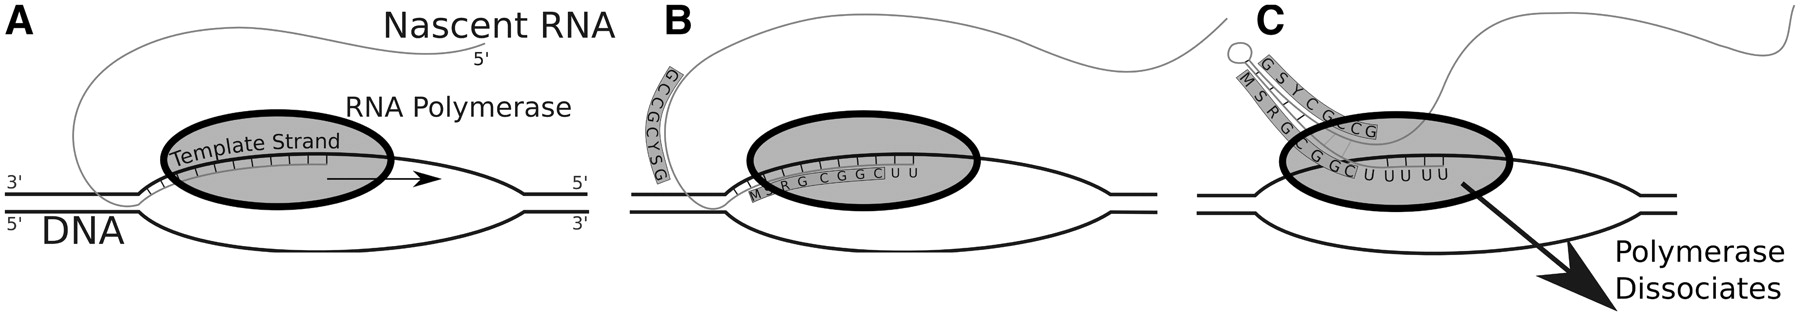
\includegraphics[width=14cm]{rhoindy.jpg}
\caption[Rho-independent termination]{\textbf{Rho-independent termination.} A) The RNA polymerase traverses the DNA template strand from $3^\prime$  to $5^\prime$ , synthesizing the nascent RNA molecule. B) As the polymerase nears a termination site, a G+C-rich terminator stem sequence (boxed) is transcribed. C) Formation of a hairpin structure causes the polymerase to pause, and together with a string of unstable rU-dA bonds causes the polymerase to release from the template. Reproduced from \textcite{Gardner2011a}.
} 
\label{fig:rho}
\end{center}
\end{figure}

\subsection{Previous approaches}
\begin{figure}[htp]
\begin{center}

\includegraphics[width=14cm]{transterm}
\caption[TransTermHP motif]{\textbf{TransTermHP motif.} Schematic of the terminator motif for which TransTermHP searches. The terminators consist of a short stem-loop hairpin followed by a thymine-rich region on their $3^\prime$ side. TransTermHP is generally restricted to find terminators for which each side of the stem is $\ge$4 nt, the length of the loop is $\ge$3 nt and $\le$13 nt, and the total length of the stem-loop was $\le$59 nt. Reproduced under a Creative Commons Attribution License (CCAL) from \textcite{Kingsford2007}.
} 
\label{fig:transterm}
\end{center}
\end{figure}
\subsection{Covariance models}

\section{Methods}

\section{Results}
\subsection{Alpha benchmark}

\begin{figure}[htp]
\begin{center}
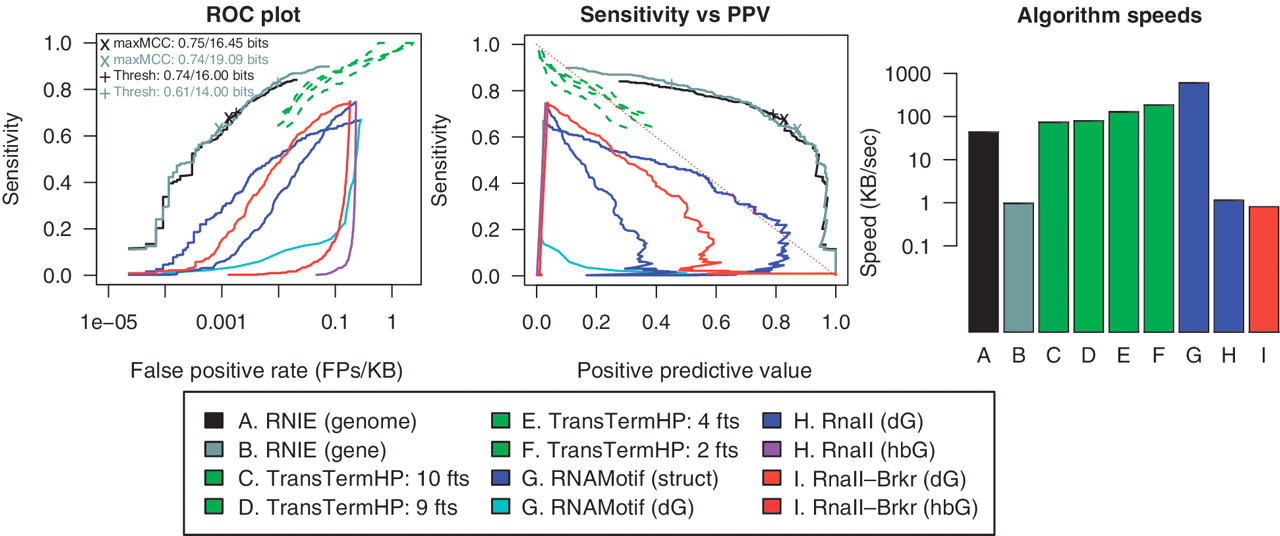
\includegraphics[width=14cm]{alpha.jpg}
\caption[Alpha benchmark]{\textbf{Alpha benchmark.} The accuracy of RNIE compared to existing methods of terminator prediction. The left figure shows a ROC plot for four independent methods. The middle figure compares the sensitivity and PPV for the four methods. The figure on the right shows the speeds for each algorithm in kilobases per second. Reproduced from \textcite{Gardner2011a}.
} 
\label{fig:alpha}
\end{center}
\end{figure}

\subsection{Beta benchmark}

\begin{figure}[htp]
\begin{center}
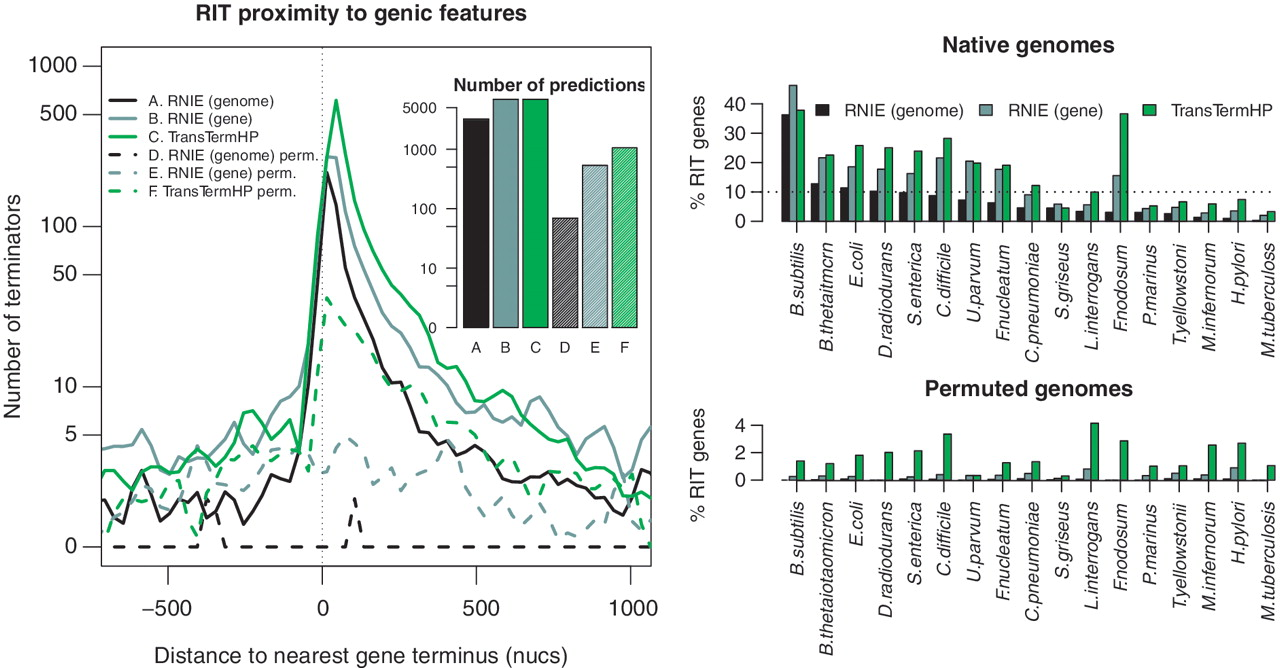
\includegraphics[width=14cm]{beta.jpg}
\caption[Beta benchmark]{\textbf{Beta benchmark.} Ideal terminator predictors will generally produce predictions that are immediately $3^\prime$ to annotated genes on native sequence and no predictions on shuffled controls. For all the test genomes in Table 1 (excluding {\it E. coli} and {\it B. subtilis}), we computed the distance to the nearest $3^\prime$ genic element, including CDSs, ncRNAs and riboswitches. This was done for both native sequences and dinucleotide shuffled control sequences with corresponding gene annotation transferred to the controls. The figure on the left shows the distribution of distances for RNIE genome and gene modes and for the TransTermHP method. Inset is a barplot showing the total number of predictions for each method on native and shuffled genomes. The figures on the right show the percentage of genes that have a predicted RIT in the region $-50$ to $+150$ from an annotated $3^\prime$-end of a CDS or ncRNA across all the genome sequences described in Table 1. The upper panel illustrates the results for the native genomes, while the lower panel illustrates results for the permuted genomes. Reproduced from \textcite{Gardner2011a}.
} 
\label{fig:beta}
\end{center}
\end{figure}

\subsection{A novel termination motif in {\it Mycobacterium tuberculosis}}

\begin{figure}[htp]
\begin{center}
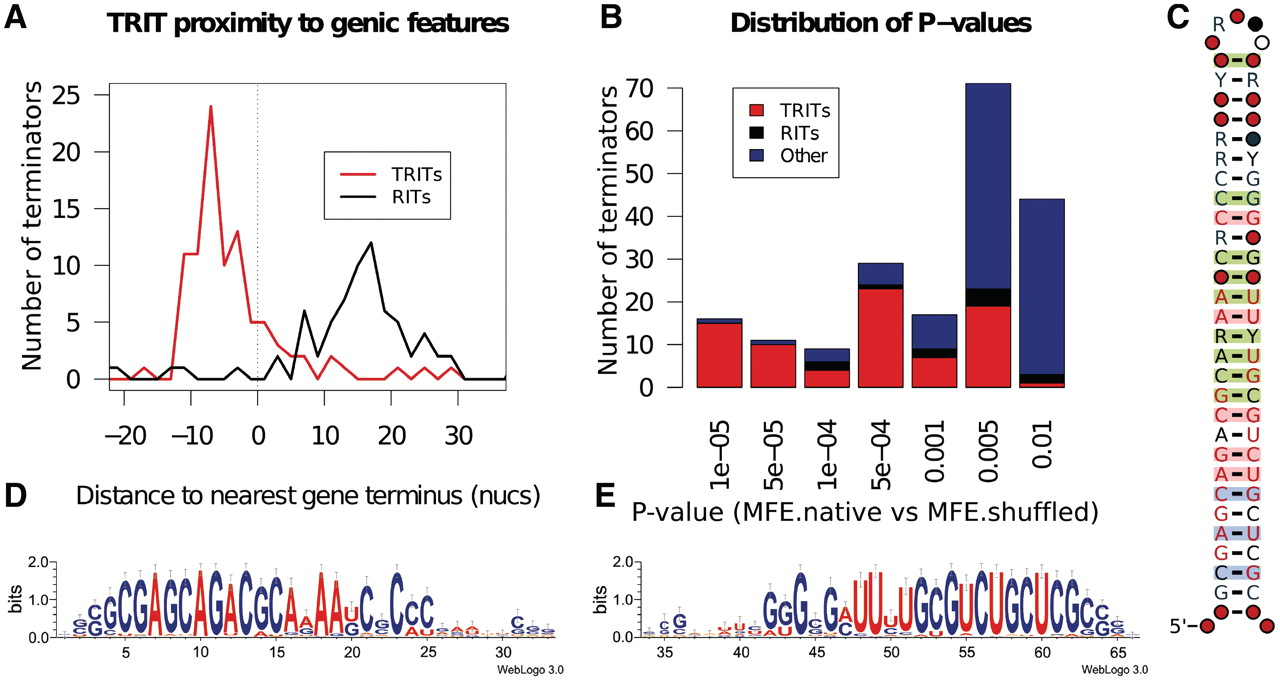
\includegraphics[width=14cm]{myco.jpg}
\caption[Putative mycobacterial transcription termination motif]{\textbf{Putative mycobacterial transcription termination motif.} A) The frequency of TRITs and RITs near the terminal regions of {\it M. tuberculosis} (EMBL accession: AE000516) genic features. B) The distribution of structural stability derived P-values for the most significant {\it M. tuberculosis} terminal regions coloured by TRIT (red), RIT (black) or unclassified (blue). C) The secondary structure and sequence conservation of the TRIT motif as displayed by R2R. (D\&E) Sequence logos generated for the $5^\prime$ D) and $3^\prime$ E) halves of an alignment of the 147 copies of TRIT in the {\it M. tuberculosis} genome. Reproduced from \textcite{Gardner2011a}.
} 
\label{fig:myco}
\end{center}
\end{figure}
